\documentclass[x11names, 12pt]{article}

% this is based on
% http://www.texample.net/tikz/examples/flexible-flow-chart/

% use half-inch margins
\usepackage[margin=0.25in]{geometry}

\usepackage[latin1]{inputenc}
\usepackage{tikz}

\usetikzlibrary{shapes,arrows,chains}

\begin{document}
\pagestyle{empty}

% -------------------------------------------------
% Set up a new layer for the debugging marks, and make sure it is on
% top
\pgfdeclarelayer{marx}
\pgfsetlayers{main,marx}

% A macro for marking coordinates (specific to the coordinate naming
% scheme used here). Swap the following 2 definitions to deactivate
% marks.
\providecommand{\cmark}[2][]{\relax}
\providecommand{\cmark}[2][]{%
  \begin{pgfonlayer}{marx}
    \node [nmark] at (c#2#1) {#2};
  \end{pgfonlayer}{marx}
  }

% -------------------------------------------------
% Start the picture
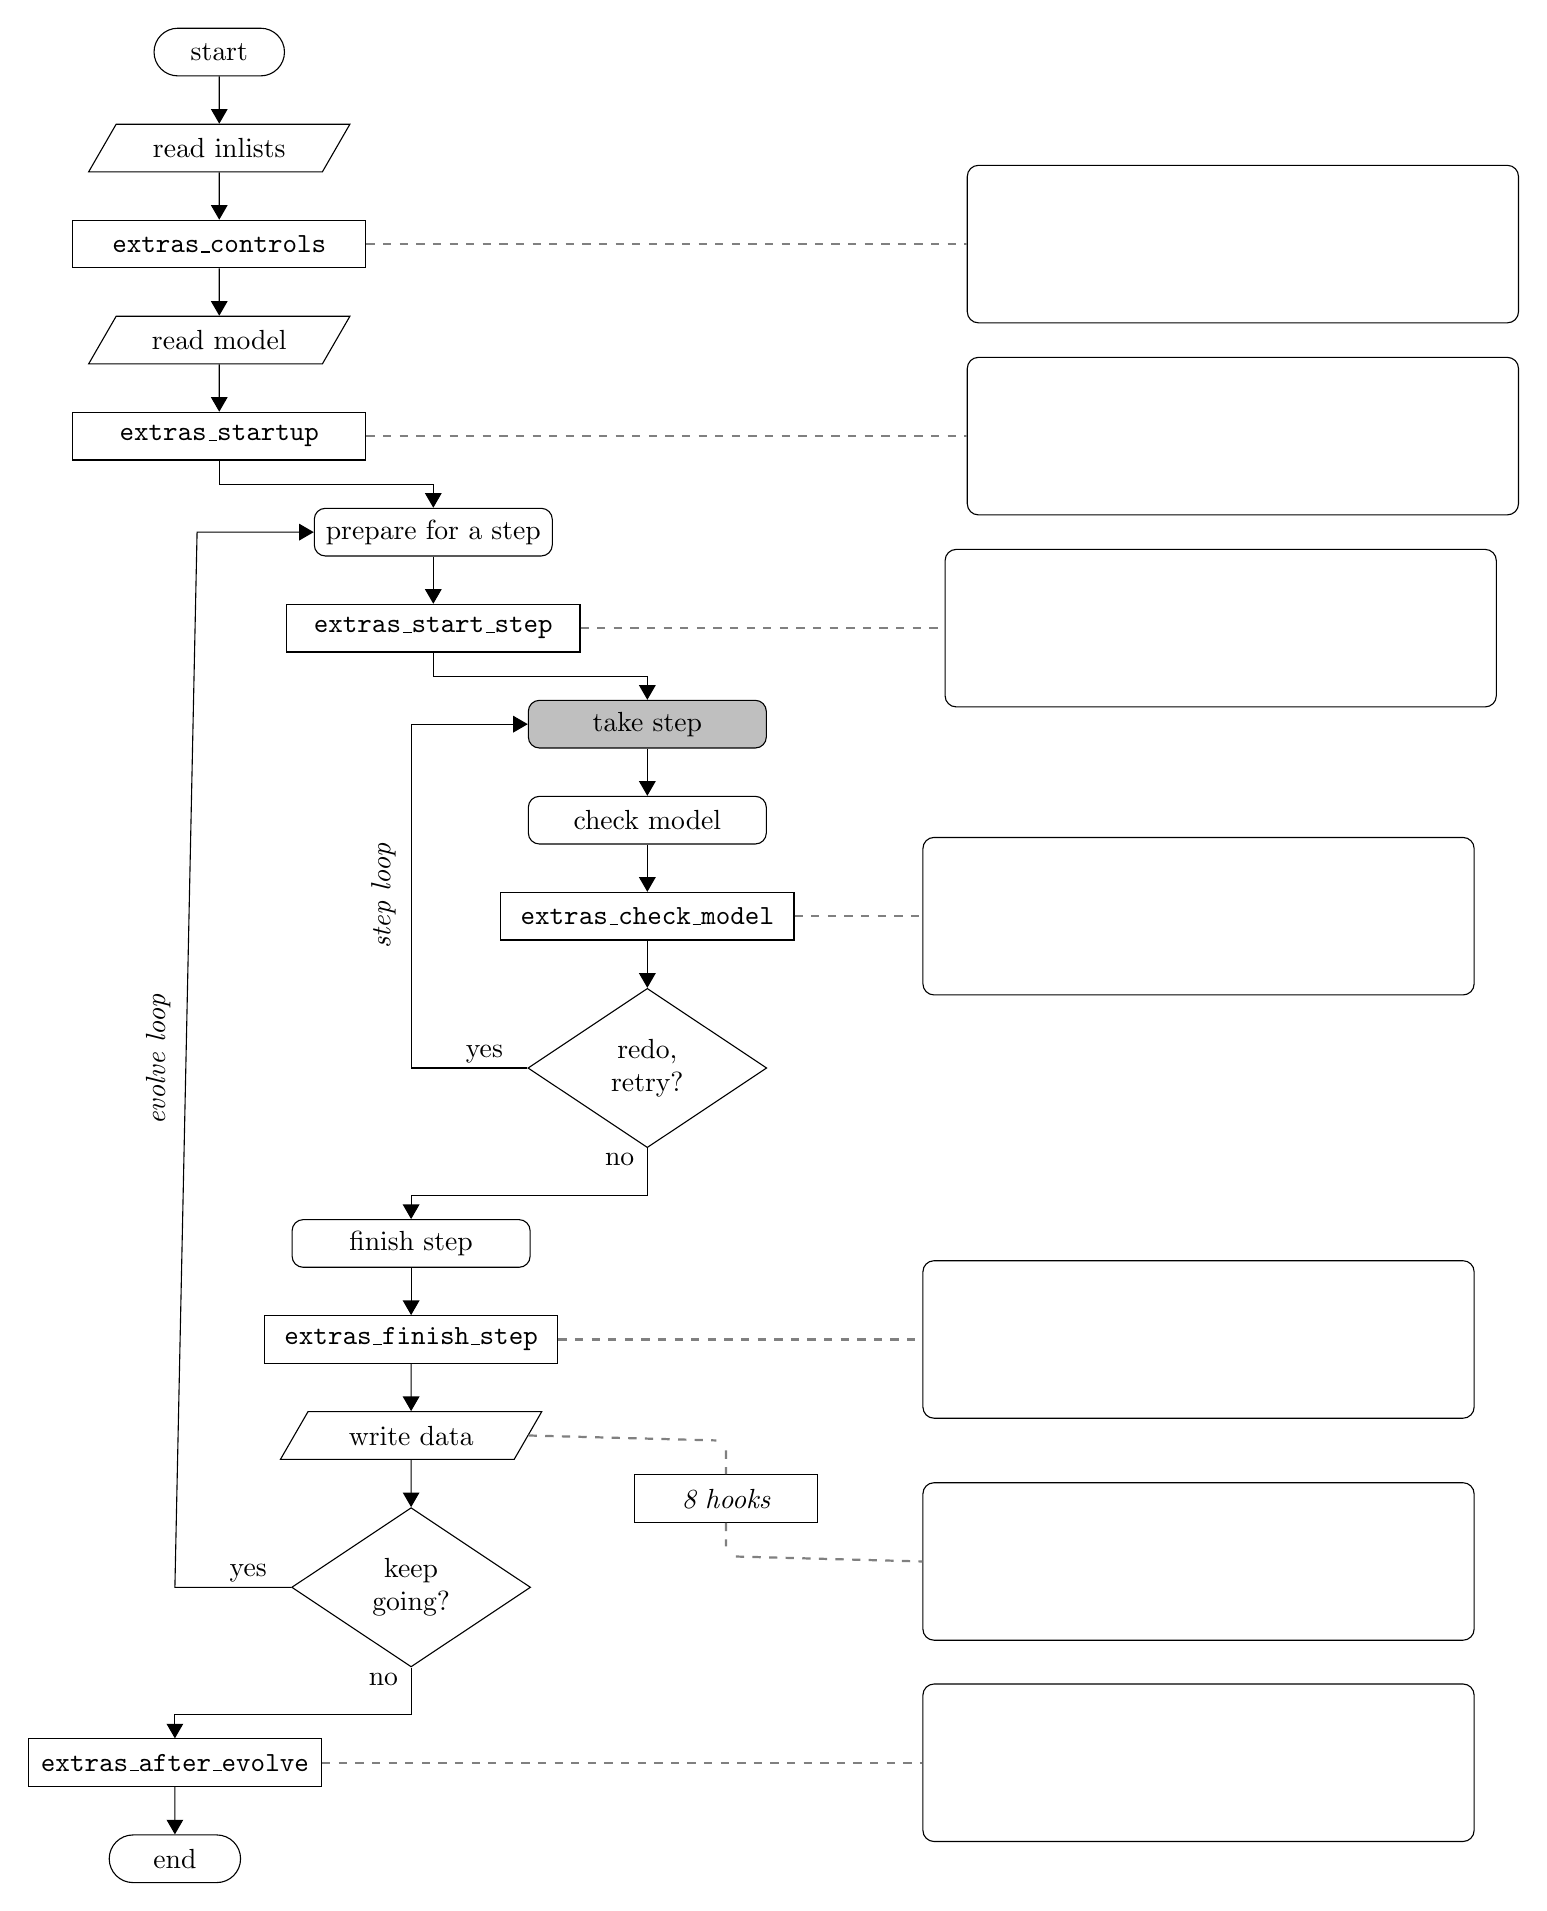
\begin{tikzpicture}[%
    >=triangle 60,              % Nice arrows; your taste may be different
    start chain=going below,    % General flow is top-to-bottom
    node distance=6mm and 12mm, % Global setup of box spacing
    every join/.style={norm},   % Default linetype for connecting boxes
    ]
% -------------------------------------------------
% A few box styles
% <on chain> *and* <on grid> reduce the need for manual relative
% positioning of nodes
\tikzset{
  base/.style={draw, on chain, on grid, align=center, minimum height=4ex, text centered, inner sep=3pt},
  endpoint/.style={base, rounded rectangle, text width=4em},
  io/.style={base, trapezium, trapezium left angle=60, trapezium right angle=-60, text width=5.0em},
  hook/.style={base, rectangle, text width = 10em},
  block/.style={base, rectangle, rounded corners, text width=8em},
  rse/.style={base, rectangle, rounded corners, minimum width=7cm, minimum height=2cm},
  decision/.style={base, diamond, aspect=1.5, text width=4em},
  % coord node style is used for placing corners of connecting lines
  coord/.style={coordinate, on chain, on grid, node distance=6mm and 12mm},
  % nmark node style is used for coordinate debugging marks
  nmark/.style={draw, cyan, circle, font={\sffamily\bfseries}},
  % -------------------------------------------------
  % Connector line styles for different parts of the diagram
  norm/.style={->, draw},
  it/.style={font={\itshape}}
}


% Start by placing the nodes

\node [endpoint] (p0) {start};
\node [io, join] (inlists) {read inlists};
\node [hook, join] (controls) {\tt extras\_controls};
\node [io, join] (model) {read model};
\node [hook, join] (startup) {\tt extras\_startup};

\node [block, below right = of startup.south] (beforestep) {prepare for a step};
\node [hook, join] (startstep) {\tt extras\_start\_step};
\node [block, fill=lightgray, below right = of startstep.south] (takestep) {take step};
\node [block, join] (check) {check model};
\node [hook, join] (checkmodel) {\tt extras\_check\_model};

\node [decision, join] (again) {redo, retry?};

\node [coord, below = of again.south] (c5)  {}; \cmark{5}
\node [coord, left = 30mm of c5] (c6)  {}; \cmark{6}

\node [block, below = 3mm of c6] (afterstep) {finish step};
\node [hook, join] (finishstep) {\tt extras\_finish\_step};
\node [io, join] (write) {write data};
\node [decision, join] (continue) {keep going?};

\node [coord, below = of continue.south] (c7)  {}; \cmark{7}
\node [coord, left = 30mm of c7] (c8)  {}; \cmark{8}

\node [hook, below = 3mm of c8] (afterevolve) {\tt extras\_after\_evolve};
\node [endpoint, join] (end) {end};

\node [rse, right = 130mm of controls] (rse_ec) {};
\node [rse, right = 130mm of startup] (rse_es) {};
\node [rse, right = 100mm of startstep] (rse_ess) {};
\node [rse, right = 70mm of checkmodel] (rse_ecm) {};
\node [rse, right = 100mm of finishstep] (rse_efs) {};
\node [rse, right = 130mm of afterevolve] (rse_eae) {};

\node [hook, text width = 6em, below right = 8 mm and 40mm of write] (write_hook) {\it 8 hooks};
\node [rse, below right = 16 mm and 100mm of write] (rse_write) {};


\draw[dashed, thick, color=gray] (controls) -- (rse_ec);
\draw[dashed, thick, color=gray] (startup) -- (rse_es);
\draw[dashed, thick, color=gray] (startstep) -- (rse_ess);
\draw[dashed, thick, color=gray] (checkmodel) -- (rse_ecm);
\draw[dashed, thick, color=gray] (finishstep) -- (rse_efs);
\draw[dashed, thick, color=gray] (afterevolve) -- (rse_eae);


\node [above = 3mm of write_hook] (d1) {};
\node [below = 3mm of write_hook] (d2) {};
\draw[dashed, thick, color=gray] (write.east) -- (d1) -- (write_hook.north);
\draw[dashed, thick, color=gray] (write_hook.south) -- (d2) -- (rse_write.west);

\node [coord, below = of continue.south] (c0) {}; \cmark{0}

\node [coord, below = of startup] (c1)  {}; \cmark{1}
\node [coord, above = of beforestep] (c2)  {}; \cmark{2}

\node [coord, below = of startstep] (c3)  {}; \cmark{3}
\node [coord, above = of takestep] (c4)  {}; \cmark{4}

\draw [->] (startup.south) -- (c1) |- (c2) -- (beforestep.north);
\draw [->] (startstep.south) -- (c3) |- (c4) -- (takestep.north);

\node [coord, left = 30mm of takestep.center] (l1)  {}; \cmark{1}
\node [coord, left = 30mm of again.center] (l2)  {}; \cmark{2}

\node [coord, left = 30mm of beforestep.center] (l3)  {}; \cmark{3}
\node [coord, left = 30mm of continue.center] (l4)  {}; \cmark{4}

\draw [->] (again.west) to node [near start, yshift=0.5em, xshift=-0.5em] {yes} (l2) to node [xshift=-1em, rotate=90, it] {step loop} (l1) -- (takestep.west);

\draw [->] (continue.west) to node [near start, yshift=0.5em, xshift=-0.5em] {yes} (l4) to node [xshift=-1em, rotate=90, it] {evolve loop} (l3) -- (beforestep.west);

\draw [->] (again.south) to node [near start, xshift=-1em] {no} (c5) -- (c6) -- (afterstep.north);
\draw [->] (continue.south) to node [near start, xshift=-1em] {no} (c7) -- (c8) -- (afterevolve.north);



\end{tikzpicture}
% =================================================
\end{document}

%%% Local Variables:
%%% mode: latex
%%% TeX-master: t
%%% End:
